\FloatBarrier
\noindent The results of Sections~\ref{sec:existence}--\ref{sec:sensitivity} were produced by a single open-source propagator written for this class of passive-sail SRP--drag problem. Because the gain regime is narrow and rests on a delicate balance between eclipse-gated SRP work and atmospheric drag, its credibility depends on two things being demonstrated independently: first, that the gain region \emph{exists} and is not an artefact of one numerical implementation; and second, that the propagator used to map it is itself trustworthy. This section addresses both by cross-validating that propagator, component by component, against two independent references: Ansys Systems Tool Kit (STK) with the Astrogator module \citep{ansysSTK2024,shortRevisitingTrajectory2019}, a widely used industry-standard flight-dynamics environment, for the conservative dynamics, the application of drag and, after two configuration corrections described below, the SRP response; and the Orekit library \citep{orekit} for the force models, the gain regime itself, and the sensitivity of the results to the atmosphere model and the solar ephemeris.

\vspace{5pt}
\par\noindent The motivation is practical as well as methodological. Solar-sail and drag-sail concepts are increasingly demonstrated in low Earth orbit on low-cost CubeSat and small-satellite platforms --- NanoSail-D \citep{johnsonNanoSailD2011}, CubeSail \citep{lappasCubeSail2011}, InflateSail \citep{underwoodInflateSail2019}, and CanX-7 \citep{boninCanX72013} --- precisely because LEO offers a cost-effective, rapidly accessible test environment for maturing sail technology before committing to expensive deep-space missions \citep{selvaCubeSatSurvey2012,woellertCubeSatCost2011}. Reliable pre-flight prediction of the coupled SRP--drag dynamics for such demonstrators requires propagation tools whose force models have been verified against a recognised reference. Open-source propagators (GMAT \citep{hughesGMATVV2014}, Orekit \citep{orekit}, poliastro \citep{canoPoliastro2022}, Basilisk \citep{kenneallyBasilisk2020}, Tudat \citep{dirkxTudatpy2022}) make such studies reproducible and inspectable, but they must be validated; cross-checking an open-source propagator against STK/HPOP is an established verification practice \citep{refaatPropagatorValidation2018,hughesGMATVV2014}.

\subsection{Open-source propagator}
\label{sec:val_propagator}
\noindent The propagator integrates the equations of motion of Section~\ref{sec:model} directly in Cartesian ECI coordinates with a fixed-step fourth-order Runge--Kutta scheme at a production step of \(10\,\mathrm{s}\) (chosen in Section~\ref{sec:val_convergence}). The force model comprises: (i) central gravity with the \(J_2\) zonal term; (ii) atmospheric drag with the frontal area \(A\lvert\cos\theta\rvert\) projected onto the instantaneous inertial velocity, no atmospheric co-rotation, and the U.S.\ Standard Atmosphere 1976 density \citep{USSA1976} evaluated at the geocentric altitude and interpolated exponentially (log-linearly) between the tabulated values (Section~\ref{sec:model}); and (iii) solar radiation pressure from a single one-sided flat plate with absorptivity \(\alpha_a = 0.3\), specular reflectivity \(\rho_s = 0.7\) and diffuse reflectivity \(\rho_d = 0\), so that the normal-incidence coefficient is \(C_r = 1.7\) (Table~\ref{tab:baseline_params}), with the solar flux scaled by \((1\,\mathrm{AU}/d_{\odot})^2\) using the analytic Sun of Section~\ref{sec:model}. A binary cylindrical umbra gates the SRP. The sail normal is constructed once, at epoch, from the LTAN, inclination and pitch angle and then frozen in inertial space, consistent with the passively spin-stabilised assumption. Mean (secular) elements are recovered by stroboscopic sampling of the osculating semi-major axis at ascending-node crossings, the first sample falling one nodal period after epoch; this removes the \(\pm 9\,\mathrm{km}\) \(J_2\) short-period signature that would otherwise mask the few-kilometre secular signal of interest. A run stops when the perigee altitude falls below \(120\,\mathrm{km}\), which is reported as re-entry.

\vspace{5pt}
\par\noindent The SRP plate uses the physically consistent specular/diffuse/absorptive decomposition of the flat-plate force \citep{mcmahonSchereesSRP2010,montenbruckGill2000}, which places the specular component along the plate normal with a \(\cos^2\alpha\) dependence, exactly the form of Eq.~\eqref{eq:srp_vector}; its agreement with the \(C_r\cos^2\alpha\) law is checked against Orekit's independent plate implementation in Section~\ref{sec:val_orekit}. We emphasise that the along-normal (specular) direction is essential: an SRP force of the same magnitude directed along the Sun line performs zero net orbit-averaged work in this geometry, because the positive and negative arcs cancel, so only the normal-directed plate reproduces the eclipse-gated pumping mechanism. Section~\ref{sec:existence} quantifies this at the gain anchor: \(\Delta a(14\,\mathrm{d}) = +5.95\,\mathrm{km}\) with the plate, \(-9.89\,\mathrm{km}\) without SRP, and \(-10.50\,\mathrm{km}\) with the Sun-line variant of the force.

\subsection{Step-size convergence}
\label{sec:val_convergence}
\noindent The umbra makes the SRP force discontinuous in time, and a fixed-step integrator that straddles the shadow boundary commits an error of first order in the step at every eclipse entry and exit. Figure~\ref{fig:convergence} shows the consequence for the \(14\)-day node-sampled \(\Delta a(14\,\mathrm{d})\) at the \(800\,\mathrm{km}\) gain anchor and at the former \(700\,\mathrm{km}\) anchor for three configurations: the full model, the full model with the umbra disabled, and drag only. At \(800\,\mathrm{km}\) the full model gives \(-1.9898\), \(+5.6508\), \(+5.9329\), \(+5.9521\), \(+5.9508\), \(+5.9546\), \(+5.9538\) and \(+5.9556\,\mathrm{km}\) at \(\Delta t = 120\), \(60\), \(30\), \(15\), \(10\), \(7.5\), \(5\) and \(2.5\,\mathrm{s}\), against \(+5.9401\,\mathrm{km}\) for an adaptive Dormand--Prince 8(5,3) (DP853) reference in Orekit with eclipse event detection, which places the integration steps exactly on the shadow boundaries. The two smooth configurations converge by \(30\,\mathrm{s}\): the umbra-disabled model gives \(-10.5934\,\mathrm{km}\) at \(30\,\mathrm{s}\) and \(-10.5873\,\mathrm{km}\) at \(10\,\mathrm{s}\) against the DP853 value of \(-10.5864\,\mathrm{km}\), and drag only gives \(-9.9091\) and \(-9.8938\,\mathrm{km}\) against \(-9.8989\,\mathrm{km}\). Running the same RK4 ladder inside Orekit confirms that the behaviour belongs to the problem, not to the implementation: a least-squares fit gives an observed convergence order of \(0.94\) for the eclipse-gated model, against the nominal fourth order, while the smooth configurations are already converged to within about \(0.01\,\mathrm{km}\) at \(30\,\mathrm{s}\) so that no meaningful order can be fitted. The coarse-step error is also non-asymptotic: in the Orekit ladder the \(60\,\mathrm{s}\) result (\(+7.229\,\mathrm{km}\)) overshoots the reference by more than the \(120\,\mathrm{s}\) result (\(+6.068\,\mathrm{km}\)), and in the present propagator the \(120\,\mathrm{s}\) step reverses the sign of the result while \(60\,\mathrm{s}\) undershoots by \(0.3\,\mathrm{km}\). Accuracy therefore cannot be inferred from the step size alone for this problem; it must be established against an event-detecting reference. The production step of \(10\,\mathrm{s}\) reproduces the DP853 reference to \(+0.18\%\) (\(+5.9508\) against \(+5.9401\,\mathrm{km}\)); at \(700\,\mathrm{km}\) the full model gives \(-21.0735\,\mathrm{km}\) at \(10\,\mathrm{s}\) against \(-21.0640\,\mathrm{km}\) at \(2.5\,\mathrm{s}\).

\begin{figure*}[htbp]
    \centering
    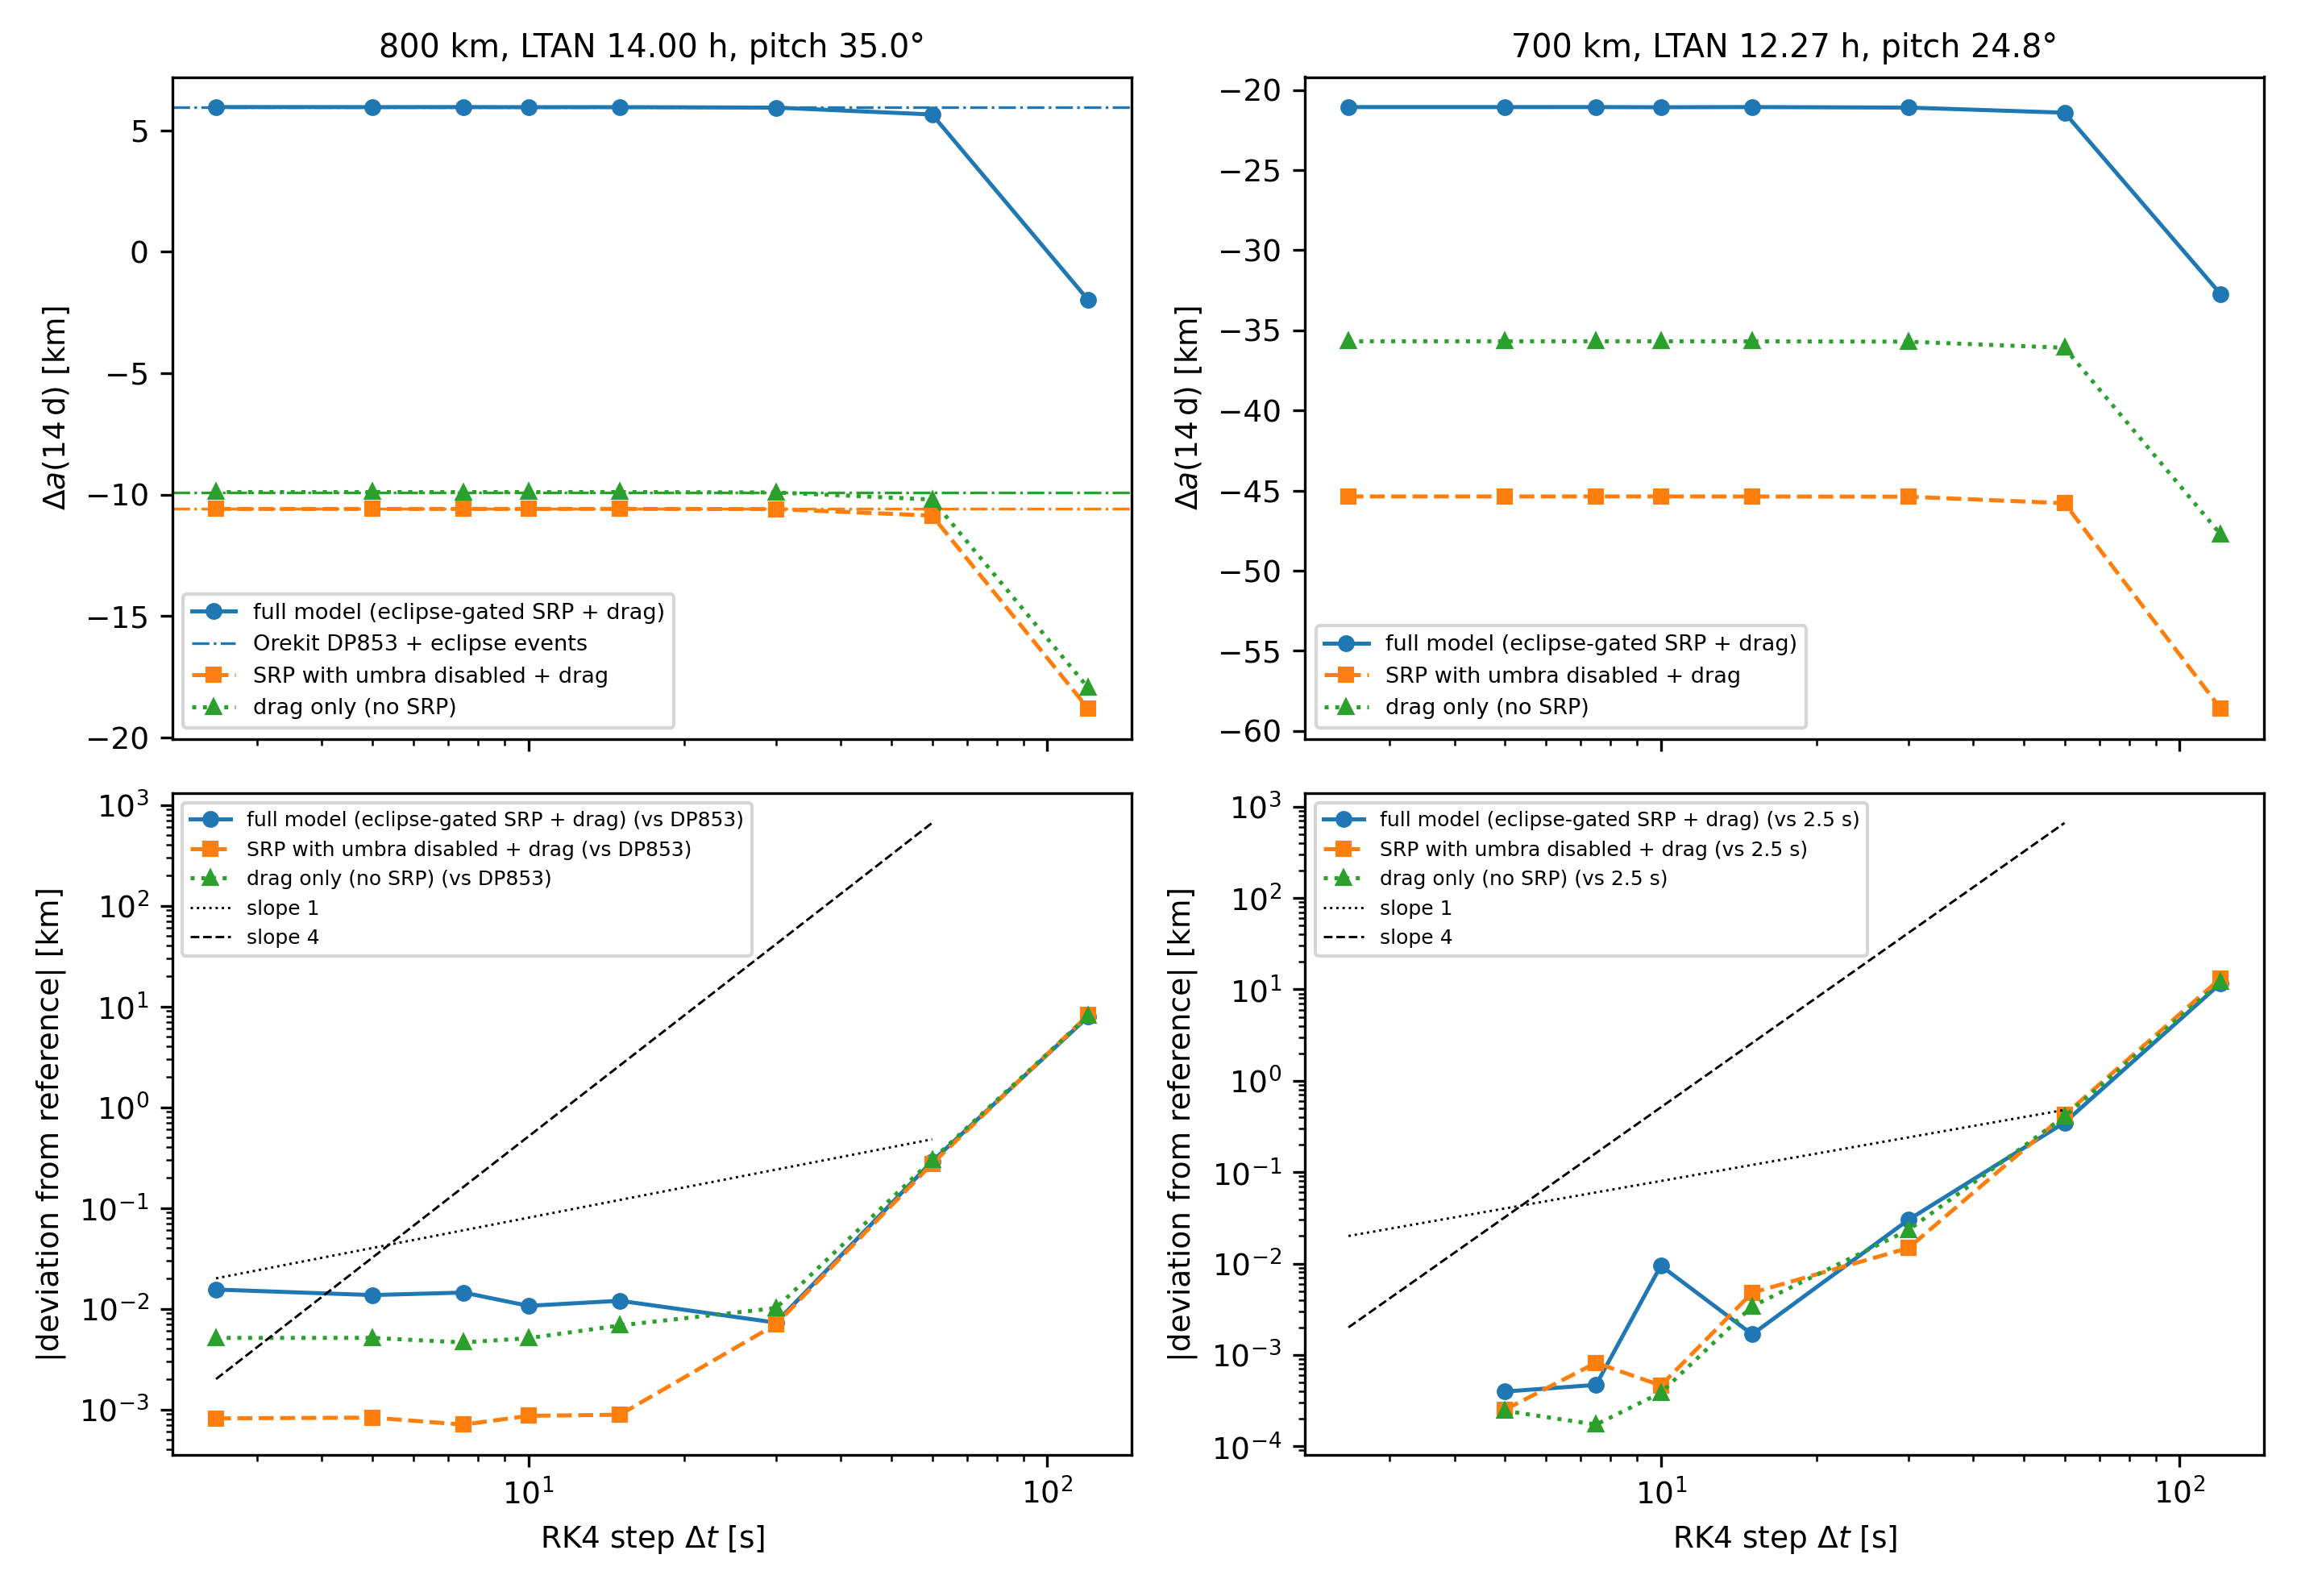
\includegraphics[width=1\linewidth]{Figures/r_convergence.png}
    \setlength{\abovecaptionskip}{0pt}
    \caption{Step-size convergence of the node-sampled \(\Delta a(14\,\mathrm{d})\) for fixed-step RK4 at \(\Delta t = 120\) to \(2.5\,\mathrm{s}\), at the \(800\,\mathrm{km}\) gain anchor (left; LTAN \(14.0\,\mathrm{h}\), pitch \(+35^\circ\)) and the former \(700\,\mathrm{km}\) anchor (right; LTAN \(12.266\,\mathrm{h}\), pitch \(+24.8^\circ\)) for the full model, the full model with the umbra disabled, and drag only. Dash-dot lines are the Orekit DP853 references with eclipse event detection at \(800\,\mathrm{km}\): \(+5.9401\), \(-10.5864\) and \(-9.8989\,\mathrm{km}\). Lower row: absolute deviation from the reference (the DP853 value at \(800\,\mathrm{km}\); the \(2.5\,\mathrm{s}\) RK4 result at \(700\,\mathrm{km}\), where no Orekit reference was run) with first- and fourth-order slope guides. The smooth configurations converge by \(30\,\mathrm{s}\); the eclipse-gated model converges only slowly (observed order about one in the Orekit ladder) and settles within \(0.02\,\mathrm{km}\) of the reference below \(15\,\mathrm{s}\); the production step of \(10\,\mathrm{s}\) reproduces the reference to \(0.18\%\).}
    \label{fig:convergence}
\end{figure*}

\subsection{STK Astrogator configuration}
\label{sec:val_stkconfig}
\noindent The STK reference cases were built with Ansys STK Engine 13.0.1 (Premium; installer \texttt{Ansys\_STK\_Premium\_\allowbreak ODTK\_v13.0.1}), driven headlessly through the \texttt{agi.stk13} Object Model from CPython 3.12 on Windows 11, so that the sweeps could be executed without the graphical interface. Each satellite uses the Astrogator propagator: a Mission Control Sequence with an Initial State segment (Keplerian elements in the Earth ICRF frame, epoch 1 Jan 2026 12:00 UTC) and a Propagate segment terminated on a Duration stopping condition. A numerical propagator cloned from ``Earth Point Mass'' carries three propagator functions configured to match the paper's model: ``Gravitational Force'' truncated to degree~2, order~0 (\(J_2\) only, tides off); ``US Standard Atmosphere'' (1976) with the spherical area model for the attitude-independent validation and the N-plate model otherwise; and ``NPlate SRP'' with the cylindrical shadow and a mean flux of \(1367.2\,\mathrm{W\,m^{-2}}\), equal to \(P_{1\,\mathrm{AU}}c\) of the open-source plate. The plate files define one body \(+Z\) SRP plate (area \(100\,\mathrm{m^2}\), specular reflectivity \(0.70\), diffuse \(0.00\)) and two opposed \(\pm Z\) drag plates (\(C_D = 2.2\)), so that the projected drag area follows \(A\lvert\cos\theta\rvert\). The inertially fixed attitude is imposed with the \texttt{eProfileFixedInAxes} profile referenced to Earth ICRF and the quaternion mapping body \(+Z\) onto the sail normal. Osculating elements are read from the Classical Elements data provider every \(60\,\mathrm{s}\); for both tools the mean semi-major axis of this comparison is the centred one-period average of the osculating value, and the quoted change is taken between \(t = T/2\) and \(t = T/2 + 14\,\mathrm{d}\), so that it spans exactly \(14\) days. (The open-source values in Table~\ref{tab:stk_validation} therefore differ slightly from the node-sampled values used elsewhere in the paper, e.g.\ \(+5.85\) against \(+5.95\,\mathrm{km}\) at the gain anchor.)

\vspace{5pt}
\par\noindent A script-based force-plugin route was attempted first and then abandoned. The Python force-model plugins of STK~13 require a registered COM server implementing the drag and SRP plugin interfaces, and registration failed on this installation. The attempt is documented in the repository, and the built-in N-plate models were used instead. Faceted and N-plate SRP models of this kind are the standard higher-fidelity representation in the flight-dynamics literature \citep{ziebartGeneralizedSRP2004,ziebartDarePixelArray2001,rodriguezsolanoBoxWing2012,vielbergRadiationPressure2020}, but they are configured through several layers of objects whose effective values are not all visible through the properties one sets; the comparison below therefore reads STK's \emph{effective} inputs back along the trajectory through the ``Astrogator Values'' data providers (applied density, drag area, SRP area, mass) rather than trusting the configured ones.

\vspace{5pt}
\par\noindent That read-back exposed two configuration errors in the STK build of the originally submitted version, which must be stated plainly because they account for its two principal findings. (i) The Initial State segment's fuel tank carried its default \(50\,\mathrm{kg}\) of fuel, which Astrogator adds to the \(10\,\mathrm{kg}\) dry mass when evaluating drag and SRP. The submitted STK runs therefore propagated a \(60\,\mathrm{kg}\) vehicle, \(A/m = 1.67\) instead of \(10\,\mathrm{m^2\,kg^{-1}}\), while every read-back property (dry mass, drag area, \(C_D\), density) looked correct because the fuel mass is stored elsewhere. This is the whole of the ``order-of-magnitude'' drag discrepancy of the submitted version (\(-7.4\,\mathrm{km}\) for STK against \(-84\,\mathrm{km}\) for the open-source propagator at \(700\,\mathrm{km}\)): with the tank zeroed, the \(14\)-day spherical-drag decay changes from \(-7.48\) to \(-60.30\,\mathrm{km}\) at \(700\,\mathrm{km}\) and from \(-2.77\) to \(-17.68\,\mathrm{km}\) at \(800\,\mathrm{km}\) (Table~\ref{tab:stk_validation}). (ii) The Object Model's \texttt{AssignQuaternion} method (interface \texttt{IAgOrientationQuaternion}) takes \((q_x, q_y, q_z, q_s)\) with the scalar component last, and had been called scalar-first. The resulting attitude mis-oriented the plate: STK's effective Sun-facing area at epoch read \(16.43\,\mathrm{m^2}\) where \(A\cos\alpha = 82.90\,\mathrm{m^2}\) was expected (probe at pitch \(34^\circ\)), and the \(3\)-day \(J_2\)+SRP response was \(+0.21\,\mathrm{km}\) against \(+3.28\,\mathrm{km}\) for the open-source propagator. This, not a limitation of the N-plate model, was the origin of the ``N-plate model does not use the attitude'' finding of the submitted version. With the Object-Model component order the effective area reads \(82.96\,\mathrm{m^2}\) and the \(3\)-day response \(+3.29\,\mathrm{km}\); at the \(35^\circ\) gain anchor the effective area is \(81.97\,\mathrm{m^2}\) (\(A\cos 35^\circ = 81.92\,\mathrm{m^2}\)), and at the former \(24.8^\circ\) anchor \(90.77\,\mathrm{m^2}\) (\(90.78\,\mathrm{m^2}\)). STK's SRP response then matches the open-source propagator, as the next subsection shows.

\subsection{Cross-validation against STK}
\label{sec:val_stk}
\noindent Figure~\ref{fig:stk_validation} and Table~\ref{tab:stk_validation} compare the two tools configuration by configuration. For the conservative dynamics (two-body plus \(J_2\), drag and SRP disabled) the centred-mean semi-major axes are identical to the metre level: the maximum absolute difference over the \(14\)-day window is \(0.25\,\mathrm{m}\) at \(700\,\mathrm{km}\) and \(0.16\,\mathrm{m}\) at \(800\,\mathrm{km}\), confirming the gravitational model, the coordinate handling and the mean-element extraction of the open-source propagator.

\vspace{5pt}
\par\noindent For \(J_2\) plus spherical drag, with the fuel tank corrected, STK gives \(-60.295\,\mathrm{km}\) against \(-70.564\,\mathrm{km}\) for the open-source propagator at \(700\,\mathrm{km}\) (ratio \(0.854\)) and \(-17.678\) against \(-18.547\,\mathrm{km}\) at \(800\,\mathrm{km}\) (ratio \(0.953\)); with the N-plate drag model at the gain-anchor attitude the corresponding values are \(-27.972\) against \(-31.524\,\mathrm{km}\) (ratio \(0.887\)) at \(700\,\mathrm{km}\) and \(-9.446\) against \(-10.015\,\mathrm{km}\) (ratio \(0.943\)) at \(800\,\mathrm{km}\). The as-submitted default-tank values of \(-7.482\) and \(-2.770\,\mathrm{km}\) are plotted dotted in panel (b) and listed in the table for the record. The residual \(5\)--\(15\%\) is a difference of convention, not of force magnitude. Astrogator applies a co-rotating atmosphere and evaluates the density at the geodetic altitude, whereas the paper's model uses the inertial velocity and the geocentric altitude. Orekit, switching these one at a time with everything else fixed (Section~\ref{sec:val_drag}), gives factors of \(\times1.034\) (co-rotation) and \(\times0.816\) (geodetic altitude) at \(700\,\mathrm{km}\), \(\times1.024\) and \(\times0.901\) at \(800\,\mathrm{km}\), and \(\times0.842\) and \(\times0.922\) combined, which accounts for the STK/open-source ratios to within about \(1.5\%\) at \(700\,\mathrm{km}\) and \(3\%\) at \(800\,\mathrm{km}\). The density STK actually applied, read back along the trajectory, averages \(0.887\) (range \(0.757\)--\(1.032\), over \(632\)--\(699\,\mathrm{km}\)) and \(0.937\) (range \(0.839\)--\(1.040\), over \(774\)--\(799\,\mathrm{km}\)) of the open-source value at the same geocentric altitude, consistent with the geodetic-altitude evaluation. For the extreme area-to-mass ratio of a sail (\(A/m = 10\,\mathrm{m^2\,kg^{-1}}\)) atmospheric drag is the dominant and least portable element of the force model \citep{anselmoHAMR2010}, and these conventions must be stated for any LEO sail prediction to be reproducible; they are now stated in Section~\ref{sec:model}.

\vspace{5pt}
\par\noindent With the quaternion corrected, STK's N-plate SRP response at the gain anchor agrees with the open-source plate: \(+15.554\) against \(+15.565\,\mathrm{km}\) over \(14\) days with eclipse on (maximum difference \(0.014\,\mathrm{km}\), about \(0.1\%\)), and \(+0.004\) against \(+0.006\,\mathrm{km}\) with the umbra removed, so both tools reproduce the cancellation of the orbit-averaged SRP work under continuous illumination that Section~\ref{sec:physics} predicts. For the full model at the gain anchor STK gives \(+6.441\,\mathrm{km}\) with eclipse on and \(-10.134\,\mathrm{km}\) with it off, against \(+5.846\) and \(-10.927\,\mathrm{km}\) for the open-source propagator: the eclipse-driven sign reversal of Section~\ref{sec:existence} is reproduced, and STK's slightly larger gain follows directly from its \(5\%\) weaker drag. Over \(75\) days STK reproduces the transient signature of Section~\ref{sec:breakdown}: its mean semi-major axis peaks at \(+12.92\,\mathrm{km}\) on day \(41.9\) and ends at \(+2.56\,\mathrm{km}\), against a peak of \(+10.60\,\mathrm{km}\) on day \(38.0\) and \(-2.70\,\mathrm{km}\) at day \(75\) for the open-source propagator under the centred-mean definition (\(+10.86\,\mathrm{km}\) on day \(38.1\) and \(-2.69\,\mathrm{km}\) node-sampled, Table~\ref{tab:cases}); the end-point difference of \(5.3\,\mathrm{km}\) is the drag-convention difference accumulated over \(1069\) orbits of decay. At the former \(700\,\mathrm{km}\) anchor the full model decays in both tools, \(-17.357\,\mathrm{km}\) in STK against \(-21.548\,\mathrm{km}\).

\begin{figure*}[htbp]
    \centering
    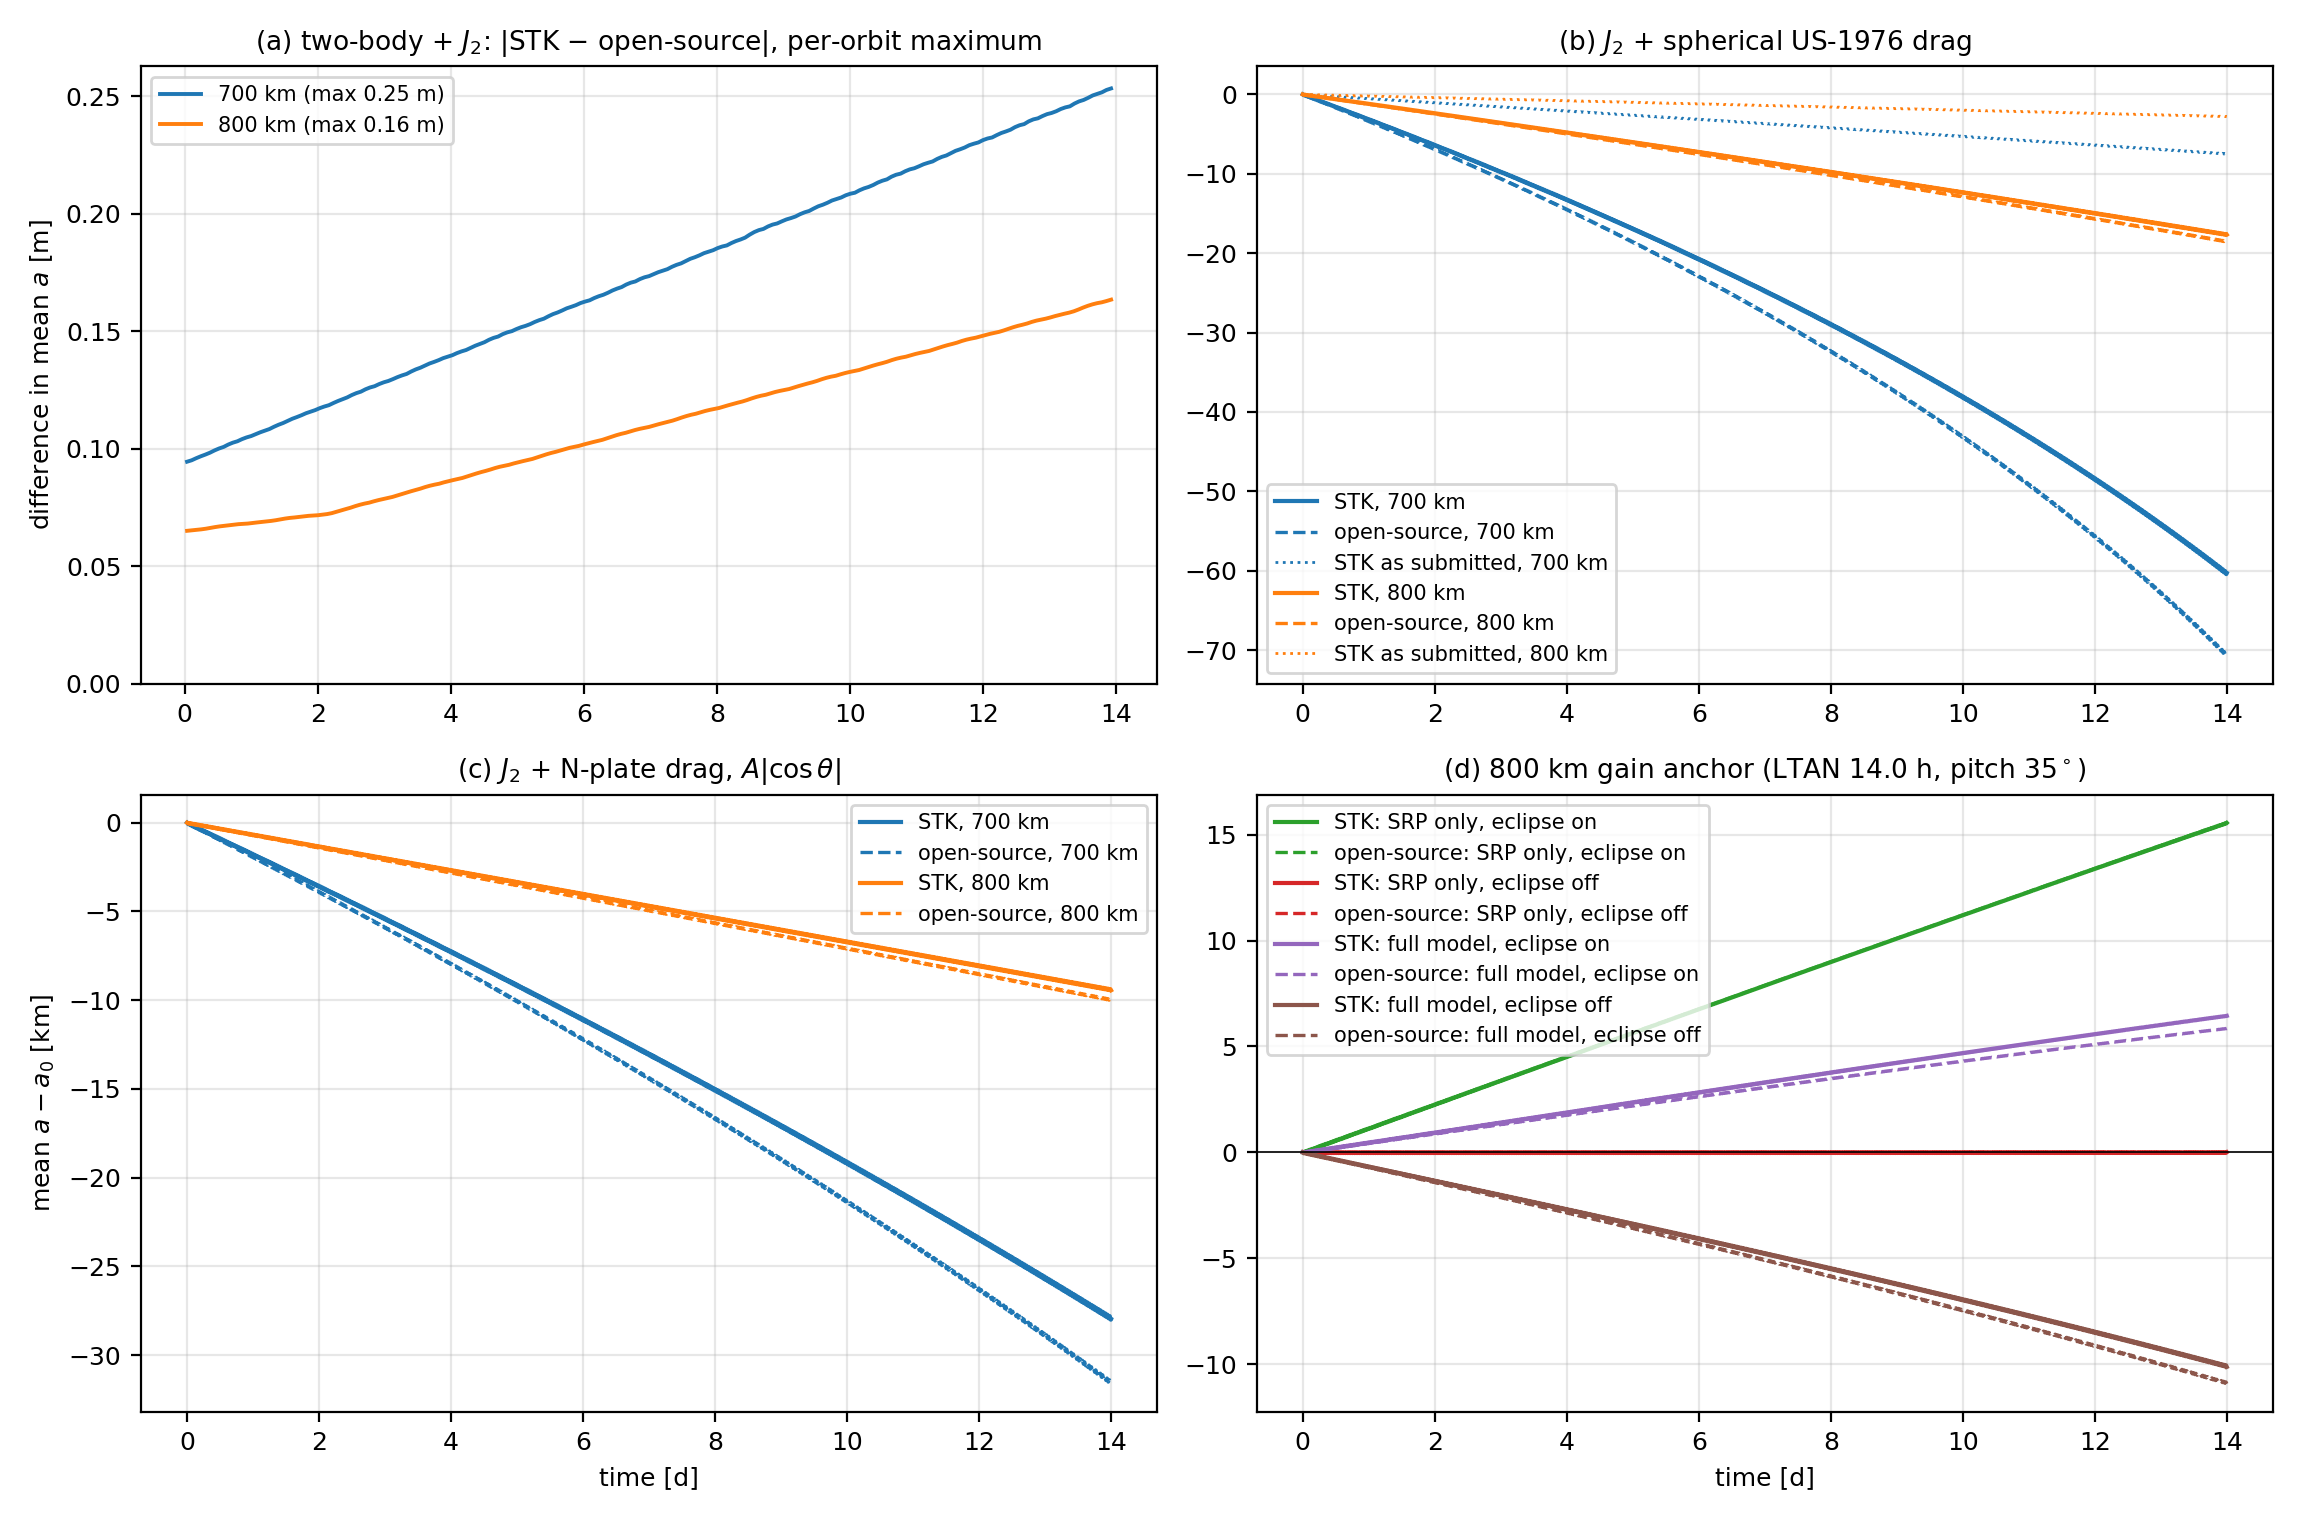
\includegraphics[width=1\linewidth]{Figures/r_stk_validation.png}
    \setlength{\abovecaptionskip}{0pt}
    \caption{Cross-validation of the open-source propagator against STK Astrogator (STK Engine 13.0.1), centred one-period mean semi-major axis over \(14\) days. (a) Two-body plus \(J_2\) at \(700\) and \(800\,\mathrm{km}\): per-orbit maximum of the absolute difference between the two tools, which stays below \(0.25\,\mathrm{m}\) over \(14\) days. (b) \(J_2\) plus spherical U.S.\ Standard Atmosphere 1976 drag with the fuel tank corrected (solid) and the as-submitted default-tank curves (dotted). (c) \(J_2\) plus N-plate drag at the gain-anchor attitude. (d) SRP only and the full model at the \(800\,\mathrm{km}\) gain anchor with eclipse on and off; the sign reversal under eclipse is reproduced by both tools.}
    \label{fig:stk_validation}
\end{figure*}

\begin{table*}[htbp]
\centering
\caption{Cross-validation against STK Astrogator: change in the centred one-period mean semi-major axis over \(14\) days (\(75\) days for the last two rows), STK against the open-source propagator (OS), the ratio STK/OS, and the maximum absolute difference \(\max\lvert\Delta\rvert\) between the two over the window; all changes in km. Gain anchor LTAN \(14.0\,\mathrm{h}\), pitch \(+35^\circ\); the former-anchor row uses LTAN \(12.266\,\mathrm{h}\), pitch \(+24.8^\circ\). The ``default tank'' rows are the build of the original submission (\(60\,\mathrm{kg}\) vehicle), shown for the record.}
\label{tab:stk_validation}
\vspace{0.5em}
\footnotesize
\setlength{\tabcolsep}{3pt}
\begin{tabular}{l c r r r r}
\toprule
Configuration & Alt.\ [km] & STK & OS & STK/OS & \(\max\lvert\Delta\rvert\) \\
\midrule
Two-body + \(J_2\) & 700 & \(-0.055\) & \(-0.055\) & \(0.999\) & \(0.0003\) \\
Two-body + \(J_2\) & 800 & \(-0.000\) & \(-0.000\) & --- & \(0.0002\) \\
\(J_2\) + spherical drag, default tank & 700 & \(-7.482\) & \(-70.564\) & \(0.106\) & \(63.196\) \\
\(J_2\) + spherical drag, default tank & 800 & \(-2.770\) & \(-18.547\) & \(0.149\) & \(15.817\) \\
\(J_2\) + spherical drag, corrected & 700 & \(-60.295\) & \(-70.564\) & \(0.854\) & \(10.535\) \\
\(J_2\) + spherical drag, corrected & 800 & \(-17.678\) & \(-18.547\) & \(0.953\) & \(0.885\) \\
\(J_2\) + N-plate drag & 700 & \(-27.972\) & \(-31.524\) & \(0.887\) & \(3.678\) \\
\(J_2\) + N-plate drag & 800 & \(-9.446\) & \(-10.015\) & \(0.943\) & \(0.571\) \\
\(J_2\) + N-plate SRP, eclipse on & 800 & \(+15.554\) & \(+15.565\) & \(0.999\) & \(0.014\) \\
\(J_2\) + N-plate SRP, eclipse off & 800 & \(+0.004\) & \(+0.006\) & \(0.758\) & \(0.002\) \\
Full model, eclipse on & 800 & \(+6.441\) & \(+5.846\) & \(1.102\) & \(0.597\) \\
Full model, eclipse off & 800 & \(-10.134\) & \(-10.927\) & \(0.927\) & \(0.796\) \\
Full model, eclipse on, former anchor & 700 & \(-17.357\) & \(-21.548\) & \(0.805\) & \(4.193\) \\
Full model, \(75\,\mathrm{d}\), peak & 800 & \(+12.922\) & \(+10.604\) & --- & --- \\
Full model, \(75\,\mathrm{d}\), final & 800 & \(+2.560\) & \(-2.695\) & --- & \(5.275\) \\
\bottomrule
\end{tabular}
\end{table*}

\subsection{Cross-validation against Orekit}
\label{sec:val_orekit}
\noindent STK validates the conservative dynamics, the application of drag and the SRP response, but its force models are closed. The second reference is therefore Orekit 13.1.7 (Hipparchus 4.0.3), driven through \texttt{orekit\_jpype}, whose force models, attitude handling, planetary ephemerides and adaptive integrators are independent of the present code and inspectable. The mapping is one-to-one: \texttt{NewtonianAttraction} and \texttt{J2OnlyPerturbation} with the paper's constants; a \texttt{FrameAlignedProvider} for the frozen sail normal; a \texttt{BoxAndSolarArraySpacecraft} with one one-sided \texttt{FixedPanel} (absorption \(0.3\), reflection \(0.7\)) for SRP through \texttt{RadiationPressureModel} with a \texttt{CylindricallyShadowedLightFluxModel}, and the same panel double-sided in a separate spacecraft for \texttt{DragForce}; \texttt{IsotropicDrag} for the spherical validation case; the paper's US-1976 interpolation injected as an Orekit \texttt{Atmosphere}, or Orekit's own Harris--Priester and NRLMSISE-00 models; and the Sun either from the paper's analytic series, to isolate the propagators, or from the JPL DE-440 ephemeris. Like-for-like comparisons use fixed-step RK4 at \(30\,\mathrm{s}\) in both tools; the reference runs use DP853 with eclipse event detection. Table~\ref{tab:orekit} collects the results.

\vspace{5pt}
\par\noindent At the level of the force models, the two implementations are the same to round-off. At \(198\) states along one orbit the maximum relative difference of the accelerations is \(0\) for gravity, \(7.4\times10^{-15}\) for drag and \(1.1\times10^{-15}\) for SRP; the eclipse flag agrees at \(198\) of \(198\) states; the plate normal recovered from Orekit's propagated attitude matches the paper's construction to \(2.8\times10^{-17}\), and the plate force follows the \(\cos^2\alpha\) law to \(1.5\times10^{-15}\). The propagated \(14\)-day mean semi-major axis (RK4 \(30\,\mathrm{s}\), spherical drag, no SRP) is then identical to within \(4\times10^{-10}\,\mathrm{km}\): \(-0.01198\,\mathrm{km}\) (\(700\,\mathrm{km}\)) and \(-0.01128\,\mathrm{km}\) (\(800\,\mathrm{km}\)) with \(J_2\) only, \(-69.872\) and \(-18.382\,\mathrm{km}\) with \(J_2\) plus drag, in both tools. The SRP attitude coupling that the submitted STK build could not exercise is confirmed by Orekit's N-plate: the effective Sun-facing area at the former \(24.8^\circ\) anchor is \(90.76\,\mathrm{m^2}\) against the analytic \(90.78\,\mathrm{m^2}\), the plate acceleration is \(80.2\,\mu\mathrm{m\,s^{-2}}\) at normal incidence and zero at \(\alpha = 90^\circ\), and over a sweep of incidence angles the N-plate magnitude departs from \(C_r\cos^2\alpha\) by at most \(1.55\%\) for \(\alpha \le 45^\circ\).

\vspace{5pt}
\par\noindent For the full model at the gain anchor the propagators agree, and the remaining difference is attributable to the Sun ephemeris. With the same analytic Sun held at \(1\,\mathrm{AU}\) in both tools (RK4 \(30\,\mathrm{s}\)), the open-source propagator gives \(\Delta a(14\,\mathrm{d}) = +5.438\,\mathrm{km}\) and Orekit \(+5.605\,\mathrm{km}\), a maximum difference along the window of \(0.181\,\mathrm{km}\); with each tool's production Sun --- the analytic series with flux \(\propto 1/d_{\odot}^2\) here, DE-440 in Orekit --- the values are \(+5.933\) and \(+6.127\,\mathrm{km}\) (maximum difference \(0.194\,\mathrm{km}\)). The Sun ephemeris alone (analytic against DE-440, everything else fixed) moves the \(14\)-day gain by \(0.522\,\mathrm{km}\), about \(9\%\), a sensitivity worth stating: the epoch lies within days of perihelion, the analytic direction departs from DE-440 by up to \(0.369^\circ\) over \(75\) days, and the Sun distance departs from \(1\,\mathrm{AU}\) by up to \(1.67\%\). At the former \(700\,\mathrm{km}\) anchor the corresponding values are \(-21.478\) against \(-21.180\,\mathrm{km}\) and \(-21.158\) against \(-20.842\,\mathrm{km}\), both decaying.

\vspace{5pt}
\par\noindent Figure~\ref{fig:repro_lobe} compares the \(800\,\mathrm{km}\) map of \(\Delta a_{\max,14\mathrm{d}}\) with its Orekit counterpart, computed with DP853 and eclipse event detection on a \(24\times19\) subset of the \(48\times37\) grid of Figure~\ref{fig:heatmap_700km} (LTAN step \(1\,\mathrm{h}\), pitch step \(10^\circ\); \(456\) common cells, none failed). Both maps have \(82\) positive cells, the sign agrees in every cell, and both peak at (\(14.0\,\mathrm{h}\), \(+30^\circ\)), the nearest common cell to the \(+35^\circ\) anchor, with \(5.776\,\mathrm{km}\) here and \(5.753\,\mathrm{km}\) in Orekit. The cell-by-cell difference has a mean of \(0.003\,\mathrm{km}\), an RMS of \(0.029\,\mathrm{km}\) (\(0.068\,\mathrm{km}\) over the positive cells) and a maximum of \(0.236\,\mathrm{km}\). The eclipse-causality test of Section~\ref{sec:existence} is reproduced over \(30\) days at the gain anchor: Orekit gives \(+10.33\,\mathrm{km}\) with eclipse on, still rising at day \(30\), and \(-28.53\,\mathrm{km}\) with it off, while the former \(700\,\mathrm{km}\) anchor gives \(-90.66\) and \(-459.0\,\mathrm{km}\). Over \(75\) days the Orekit gain case peaks at \(+10.95\,\mathrm{km}\) on day \(37.9\) and ends at \(-2.37\,\mathrm{km}\) with \(e = 0.01225\), apogee \(885.6\,\mathrm{km}\) and perigee \(709.7\,\mathrm{km}\), against \(+10.86\,\mathrm{km}\) on day \(38.1\), \(-2.69\,\mathrm{km}\), \(e = 0.0122\), \(884.7\) and \(709.9\,\mathrm{km}\) in Table~\ref{tab:gaincase_longhorizon_summary}; the Orekit propagation of the former \(700\,\mathrm{km}\) anchor ends on day \(39.3\) at \(-412.5\,\mathrm{km}\) with the perigee at \(275\,\mathrm{km}\), the counterpart of the re-entry on day \(39.5\) in Table~\ref{tab:cases}. The one-orbit SRP work budget of Figures~\ref{srp_vs_anomaly} and \ref{cum_SRP} is reproduced as well: Orekit's umbra occupies \(32.0\%\) of the gain-anchor orbit (\(32.1\%\) here), \(77.6\%\) of the eclipsed samples carry negative no-eclipse SRP power (\(77.4\%\)), and the cumulative SRP work over the orbit is \(+309.7\,\mathrm{J\,kg^{-1}}\) with eclipse on and \(+0.77\,\mathrm{J\,kg^{-1}}\) with it off (\(+310.3\) and \(+1.4\,\mathrm{J\,kg^{-1}}\)).

\vspace{5pt}
\par\noindent In summary, Orekit validates the drag law, the SRP attitude coupling, the eclipse gating and the gain regime itself independently of the present implementation, and STK validates the conservative dynamics, the application of drag and, with the corrected configuration, the SRP response. The regime is a property of the dynamics, not of one code.

\begin{figure*}[htbp]
    \centering
    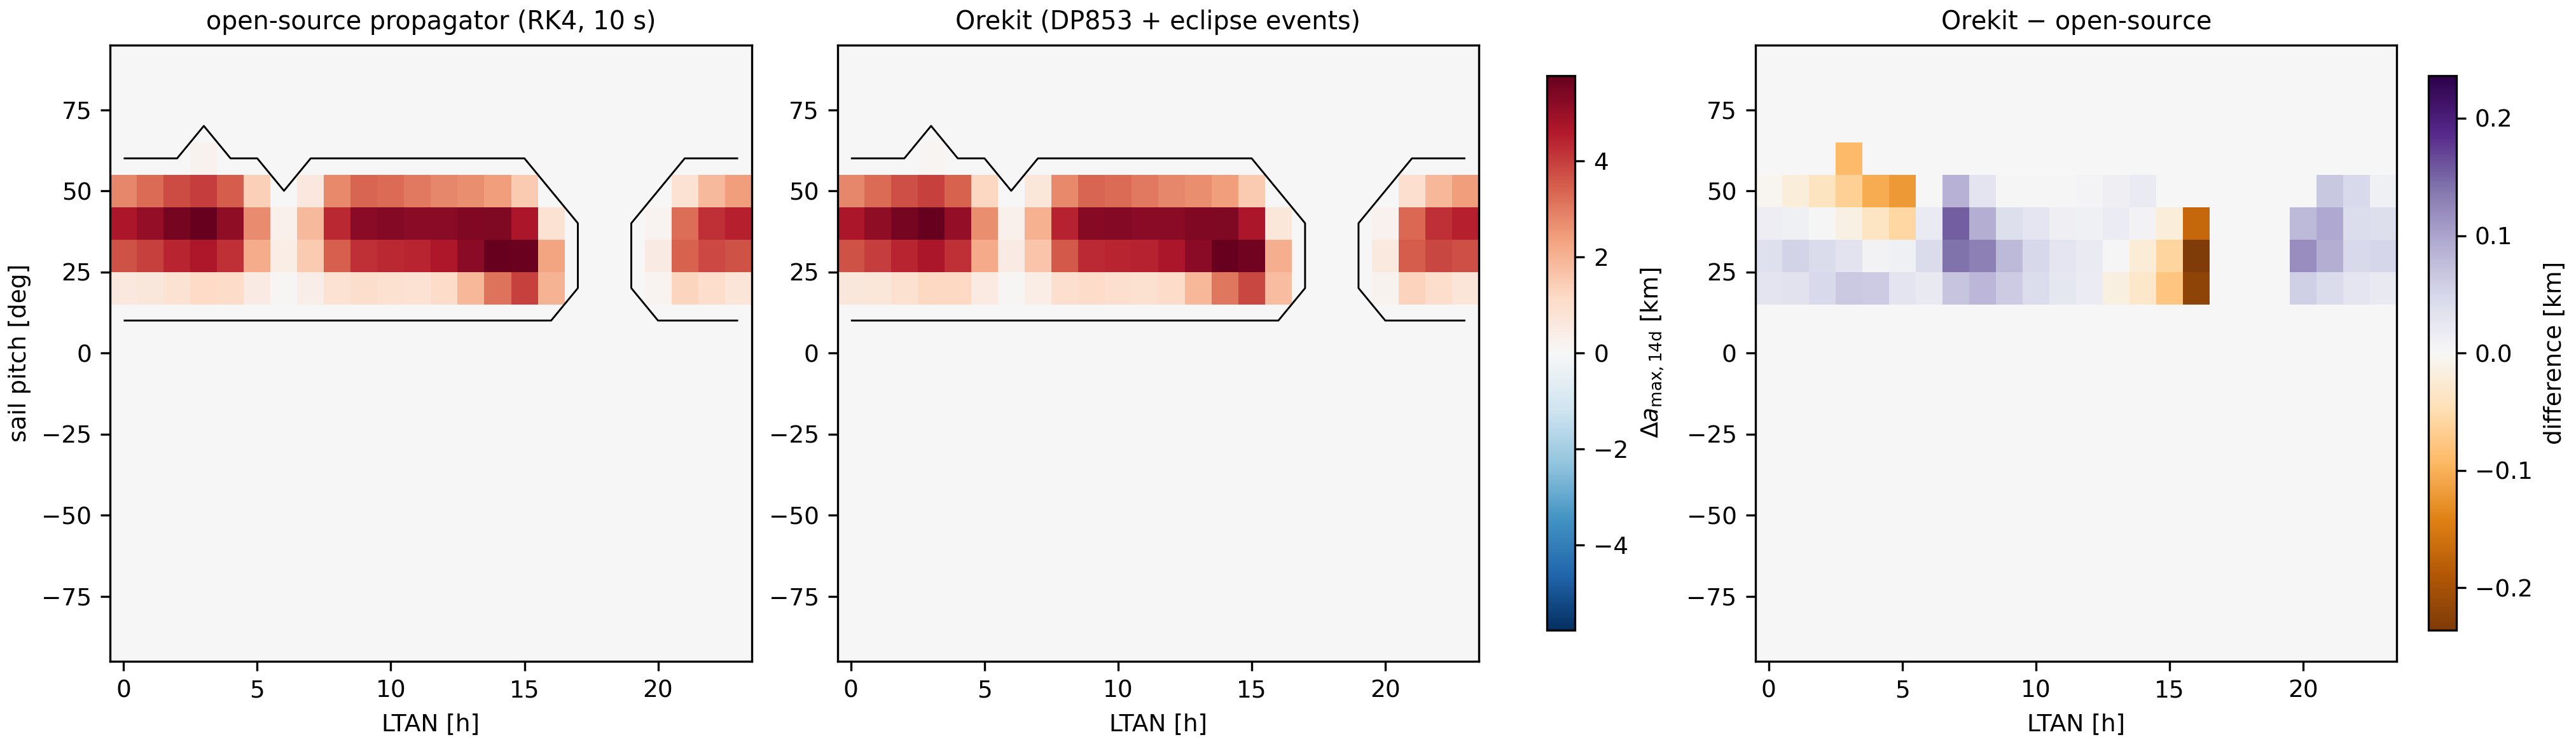
\includegraphics[width=1\linewidth]{Figures/r_map_orekit_compare.png}
    \setlength{\abovecaptionskip}{0pt}
    \caption{Independent reproduction of the \(800\,\mathrm{km}\) gain lobe. Left: \(\Delta a_{\max,14\mathrm{d}}\) from the open-source propagator on the \(24\times19\) cells common to the Orekit sweep (LTAN step \(1\,\mathrm{h}\), pitch step \(10^\circ\)). Centre: the same map from Orekit (DP853 with eclipse event detection). Right: the cell-by-cell difference (Orekit minus open-source). Both maps contain \(82\) positive cells, agree in sign everywhere and peak at LTAN \(14.0\,\mathrm{h}\), pitch \(+30^\circ\) (\(5.776\) and \(5.753\,\mathrm{km}\)); the RMS difference is \(0.029\,\mathrm{km}\) and the largest \(0.236\,\mathrm{km}\).}
    \label{fig:repro_lobe}
\end{figure*}

\begin{table*}[htbp]
\centering
\caption{Cross-validation against Orekit 13.1.7. Force gates are evaluated at \(198\) states along one orbit with a shared Sun position; propagated \(14\)-day values use RK4 at \(30\,\mathrm{s}\) in both tools and the node-sampled mean semi-major axis; the map, \(75\)-day and one-orbit rows use Orekit's DP853 integrator with eclipse event detection. Anchor LTAN \(14.0\,\mathrm{h}\), pitch \(+35^\circ\) unless stated.}
\label{tab:orekit}
\vspace{0.5em}
\footnotesize
\setlength{\tabcolsep}{3pt}
\begin{tabular}{>{\raggedright\arraybackslash}p{5.0cm} >{\raggedright\arraybackslash}p{2.4cm} >{\raggedright\arraybackslash}p{2.4cm} >{\raggedright\arraybackslash}p{2.8cm}}
\toprule
Quantity & Open-source & Orekit & Difference \\
\midrule
Gravity acceleration, relative & --- & --- & \(0\) \\
Drag acceleration, relative & --- & --- & \(7.4\times10^{-15}\) \\
SRP acceleration, relative & --- & --- & \(1.1\times10^{-15}\) \\
Eclipse flag & --- & --- & \(0\) mismatches \\
Sail normal from attitude & --- & --- & \(2.8\times10^{-17}\) \\
Plate force vs \(\cos^2\alpha\) law & --- & --- & \(1.5\times10^{-15}\) \\
\(J_2\) only, \(14\,\mathrm{d}\), \(700\,\mathrm{km}\) [km] & \(-0.01198\) & \(-0.01198\) & \(2.6\times10^{-10}\) \\
\(J_2\) only, \(14\,\mathrm{d}\), \(800\,\mathrm{km}\) [km] & \(-0.01128\) & \(-0.01128\) & \(2.7\times10^{-10}\) \\
\(J_2\) + spherical drag, \(14\,\mathrm{d}\), \(700\,\mathrm{km}\) [km] & \(-69.872\) & \(-69.872\) & \(4.0\times10^{-10}\) \\
\(J_2\) + spherical drag, \(14\,\mathrm{d}\), \(800\,\mathrm{km}\) [km] & \(-18.382\) & \(-18.382\) & \(2.8\times10^{-10}\) \\
Sun-facing area at pitch \(24.8^\circ\) [m\(^2\)] & \(90.78\) (analytic) & \(90.76\) & \(0.02\) \\
N-plate magnitude vs \(C_r\cos^2\alpha\), \(\alpha \le 45^\circ\) & --- & --- & \(\le 1.55\%\) \\
Full model, analytic Sun at \(1\,\mathrm{AU}\) [km] & \(+5.438\) & \(+5.605\) & \(0.181\) (max) \\
Full model, production Sun (\(1/d_{\odot}^2\) / DE-440) [km] & \(+5.933\) & \(+6.127\) & \(0.194\) (max) \\
Former \(700\,\mathrm{km}\) anchor, analytic Sun [km] & \(-21.478\) & \(-21.180\) & \(0.299\) (max) \\
Former \(700\,\mathrm{km}\) anchor, production Sun [km] & \(-21.158\) & \(-20.842\) & \(0.318\) (max) \\
\(800\,\mathrm{km}\) map, \(456\) common cells: positive cells & \(82\) & \(82\) & sign agreement \(100\%\) \\
\quad peak at (\(14.0\,\mathrm{h}\), \(+30^\circ\)) [km] & \(5.776\) & \(5.753\) & RMS \(0.029\), max \(0.236\) \\
\(75\,\mathrm{d}\): peak [km] (day) & \(+10.86\) (\(38.1\)) & \(+10.95\) (\(37.9\)) & \(0.09\) \\
\(75\,\mathrm{d}\): final [km] & \(-2.69\) & \(-2.37\) & \(0.32\) \\
One orbit: umbra fraction & \(32.1\%\) & \(32.0\%\) & \(0.1\%\) \\
One orbit: sign-selectivity & \(77.4\%\) & \(77.6\%\) & \(0.2\%\) \\
One orbit: SRP work, eclipse on [J\,kg\(^{-1}\)] & \(+310.3\) & \(+309.7\) & \(0.6\) \\
One orbit: SRP work, eclipse off [J\,kg\(^{-1}\)] & \(+1.4\) & \(+0.77\) & \(0.6\) \\
\bottomrule
\end{tabular}
\end{table*}

\subsection{Drag conventions and atmosphere models}
\label{sec:val_drag}
\noindent The STK comparison leaves drag as the one component whose propagated effect differs between tools, and Section~\ref{sec:sensitivity} shows that the regime boundary at \(800\,\mathrm{km}\) lies within a factor of two of the US-1976 density. Table~\ref{tab:drag_conventions} therefore separates the drag conventions from the atmosphere model with Orekit, propagating \(J_2\) plus spherical drag for \(14\) days (RK4 \(30\,\mathrm{s}\), node-sampled) and changing one element at a time. At \(700\,\mathrm{km}\) the baseline (US-1976, geocentric altitude, no co-rotation) gives \(-69.87\,\mathrm{km}\); a rigidly co-rotating atmosphere gives \(\times1.034\), the geodetic altitude \(\times0.816\), and the two together \(\times0.842\). At \(800\,\mathrm{km}\) the baseline is \(-18.38\,\mathrm{km}\) and the factors are \(\times1.024\), \(\times0.901\) and \(\times0.922\). The conventions are thus worth \(8\)--\(16\%\), and they account for the STK residual of Section~\ref{sec:val_stk} to within a few per cent. The atmosphere model is worth far more. Orekit's built-in Harris--Priester model multiplies the decay by \(7.08\) at \(700\,\mathrm{km}\), where the sail re-enters on day \(10.45\), and by \(3.15\) at \(800\,\mathrm{km}\); NRLMSISE-00 driven by the CSSI space-weather file for January 2026 multiplies it by \(2.57\) and \(1.59\). Because Orekit's built-in models are evaluated with their own conventions (geodetic altitude and co-rotation), these factors include the \(\times0.84\)--\(0.92\) convention effect, and the model effect proper is slightly larger.

\vspace{5pt}
\par\noindent A propagator-free check settles the question of scale raised by the reviewers. Integrating the secular rate \(\mathrm{d}a/\mathrm{d}t = -\rho\,C_D\,(A/m)\sqrt{\mu a}\) with the same density table along the decaying orbit gives \(-63.9\,\mathrm{km}\) at \(700\,\mathrm{km}\) and \(-17.6\,\mathrm{km}\) at \(800\,\mathrm{km}\), within \(8.5\%\) and \(4.2\%\) of the propagated \(-69.87\) and \(-18.38\,\mathrm{km}\); the remainder is the growth of eccentricity and the node-sampling convention. Holding the density at its \(700\,\mathrm{km}\) value instead gives about \(-43\,\mathrm{km}\), which is the reviewers' estimate: the difference is the density increase along the \(60\)--\(70\,\mathrm{km}\) of decay, not a defect of either tool. The three figures of the original submission are therefore reconciled as follows: \(-43\,\mathrm{km}\) is the constant-density estimate, \(-84\,\mathrm{km}\) was the value of the open-source propagator before the correction of the atmosphere table (Section~\ref{sec:model}), and \(-7\,\mathrm{km}\) was STK propagating a \(60\,\mathrm{kg}\) vehicle; the corrected values are \(-70\,\mathrm{km}\) (open-source, Orekit) and \(-60\,\mathrm{km}\) (STK, with its own conventions). At this altitude drag wins for every geometry (Figure~\ref{fig:heatmap_700km}) and the former anchor re-enters on day \(39.5\) (Table~\ref{tab:cases}).

\begin{table*}[htbp]
\centering
\caption{Drag conventions and atmosphere models in Orekit: \(14\)-day change of the node-sampled mean semi-major axis for \(J_2\) plus spherical drag (\(A/m = 10\,\mathrm{m^2\,kg^{-1}}\), \(C_D = 2.2\), RK4 at \(30\,\mathrm{s}\)), with the factor relative to the baseline of the paper (US-1976, geocentric altitude, no co-rotation). Orekit's built-in models use their own conventions (geodetic altitude, co-rotation); NRLMSISE-00 is driven by the CSSI space-weather file for January 2026. With Harris--Priester the \(700\,\mathrm{km}\) sail re-enters on day \(10.45\). The last row is the propagator-free secular integral with the same density table.}
\label{tab:drag_conventions}
\vspace{0.5em}
\footnotesize
\setlength{\tabcolsep}{4pt}
\begin{tabular}{l r r r r}
\toprule
& \multicolumn{2}{c}{\(700\,\mathrm{km}\)} & \multicolumn{2}{c}{\(800\,\mathrm{km}\)} \\
\cmidrule(lr){2-3} \cmidrule(lr){4-5}
Configuration & \(\Delta a(14\,\mathrm{d})\) [km] & factor & \(\Delta a(14\,\mathrm{d})\) [km] & factor \\
\midrule
Baseline (conventions of the paper) & \(-69.87\) & \(1.000\) & \(-18.38\) & \(1.000\) \\
Co-rotating atmosphere & \(-72.28\) & \(1.034\) & \(-18.82\) & \(1.024\) \\
Geodetic altitude & \(-57.04\) & \(0.816\) & \(-16.57\) & \(0.901\) \\
Co-rotating + geodetic & \(-58.82\) & \(0.842\) & \(-16.95\) & \(0.922\) \\
Harris--Priester (Orekit) & \(-494.7^{\dagger}\) & \(7.08\) & \(-57.84\) & \(3.15\) \\
NRLMSISE-00 (Orekit) & \(-179.9\) & \(2.57\) & \(-29.17\) & \(1.59\) \\
Analytic secular integral & \(-63.9\) & \(0.915\) & \(-17.6\) & \(0.958\) \\
\bottomrule
\end{tabular}
\par\vspace{2pt}
{\footnotesize \(^{\dagger}\)At re-entry, day \(10.45\).}
\end{table*}

\vspace{5pt}
\par\noindent The US-1976 profile is a static reference that carries no dependence on solar or geomagnetic activity (Section~\ref{sec:model}). To locate the regime boundary under a realistic thermosphere, the full model at the gain anchor was propagated for \(14\) days with the US-1976 baseline and with NRLMSISE-00 at constant low, moderate and high activity (\(F_{10.7} = 70\), \(140\) and \(200\); \(A_p = 4\), \(15\) and \(40\)) and with the CSSI space-weather file, at \(800\) and \(700\,\mathrm{km}\); Figure~\ref{fig:space_weather} and Table~\ref{tab:space_weather} report \(\Delta a_{\max,14\mathrm{d}}\) and \(\Delta a(14\,\mathrm{d})\).

\vspace{5pt}
\par\noindent At the \(800\,\mathrm{km}\) gain anchor the regime survives every atmosphere except the high-activity one. Under low activity (\(F_{10.7} = 70\), \(A_p = 4\)) the \(14\)-day gain rises to \(+13.18\,\mathrm{km}\), against \(+5.94\,\mathrm{km}\) with US-1976; under moderate activity (\(140\), \(15\)) it falls to \(+2.22\,\mathrm{km}\), with the CSSI space-weather file for January 2026 to \(+0.50\,\mathrm{km}\), and under high activity (\(200\), \(40\)) there is no gain at all (\(\Delta a_{\max,14\mathrm{d}} = 0\), \(\Delta a(14\,\mathrm{d}) = -45.5\,\mathrm{km}\)). The drag-only decays of the same runs, \(-2.33\), \(-9.90\), \(-12.72\), \(-14.43\) and \(-59.58\,\mathrm{km}\) respectively, show the cause: at this altitude and geometry the low-activity NRLMSISE-00 drag is about a quarter of the US-1976 value, the moderate level and the January 2026 file about \(1.3\) and \(1.5\) times it, and the high level about six times. At \(700\,\mathrm{km}\) the same geometry gains only under low activity (\(+10.69\,\mathrm{km}\); drag only \(-4.69\,\mathrm{km}\)); it decays with US-1976 (\(-13.77\,\mathrm{km}\); \(-31.15\,\mathrm{km}\) drag only), under moderate activity (\(-30.87\); \(-45.15\,\mathrm{km}\)) and with the CSSI file (\(-38.52\); \(-52.78\,\mathrm{km}\)), and under high activity it re-enters within the \(14\) days both with and without SRP.

\vspace{5pt}
\par\noindent The regime boundary therefore moves with the thermosphere. At \(800\,\mathrm{km}\) the gain survives under low and moderate activity, is marginal under the January 2026 conditions and closes under high activity; at \(700\,\mathrm{km}\) it exists only under low activity, where the quiet-Sun thermosphere is thinner than the static US-1976 profile. The US-1976 baseline of this paper thus lies between the low and moderate NRLMSISE-00 levels and slightly below the January 2026 conditions: it is neither the most favourable nor the least favourable case. The NRLMSISE-00 runs use Orekit's implementation with its own conventions (geodetic altitude, co-rotating atmosphere), and all runs use the DP853 integrator with eclipse event detection, so the US-1976 row of Table~\ref{tab:space_weather} is the DP853 reference of Section~\ref{sec:val_convergence} (\(+5.94\,\mathrm{km}\)) rather than the RK4 value of the maps.

\begin{table*}[htbp]
\centering
\caption{Space-weather dependence of the gain regime (Orekit, DP853 with eclipse event detection, \(14\) days, node-sampled mean semi-major axis): the full model and drag only at the gain-anchor geometry (LTAN \(14.0\,\mathrm{h}\), pitch \(+35^\circ\)) at \(800\) and \(700\,\mathrm{km}\) with the US-1976 baseline (conventions of the paper) and with Orekit's NRLMSISE-00 (geodetic altitude, co-rotation) at constant low, moderate and high activity (bracketed values are \(F_{10.7}\) and \(A_p\)) and with the CSSI space-weather file for January 2026. All values in km; for the full model \(\Delta a_{\max,14\mathrm{d}}\) / \(\Delta a(14\,\mathrm{d})\), for drag only \(\Delta a(14\,\mathrm{d})\). ``Re-entry'' marks runs whose perigee fell below \(120\,\mathrm{km}\) within the \(14\) days.}
\label{tab:space_weather}
\vspace{0.5em}
\footnotesize
\setlength{\tabcolsep}{3pt}
\begin{tabular}{>{\raggedright\arraybackslash}p{3.0cm} c r c r}
\toprule
& \multicolumn{2}{c}{\(800\,\mathrm{km}\)} & \multicolumn{2}{c}{\(700\,\mathrm{km}\)} \\
\cmidrule(lr){2-3} \cmidrule(lr){4-5}
Atmosphere model (activity) & full model & drag only & full model & drag only \\
& \(\Delta a_{\max,14\mathrm{d}}\) / \(\Delta a(14\,\mathrm{d})\) & \(\Delta a(14\,\mathrm{d})\) & \(\Delta a_{\max,14\mathrm{d}}\) / \(\Delta a(14\,\mathrm{d})\) & \(\Delta a(14\,\mathrm{d})\) \\
\midrule
US-1976 (baseline) & \(+5.940\) / \(+5.940\) & \(-9.899\) & \(0\) / \(-13.766\) & \(-31.152\) \\
NRLMSISE-00, low (70, 4) & \(+13.178\) / \(+13.178\) & \(-2.327\) & \(+10.685\) / \(+10.685\) & \(-4.685\) \\
NRLMSISE-00, moderate (\(140\), \(15\)) & \(+2.215\) / \(+2.213\) & \(-12.724\) & \(0\) / \(-30.872\) & \(-45.154\) \\
NRLMSISE-00, high (\(200\), \(40\)) & \(0\) / \(-45.455\) & \(-59.583\) & re-entry & re-entry \\
NRLMSISE-00, CSSI (Jan 2026) & \(+0.500\) / \(+0.499\) & \(-14.426\) & \(0\) / \(-38.517\) & \(-52.777\) \\
\bottomrule
\end{tabular}
\end{table*}

\begin{figure*}[htbp]
    \centering
    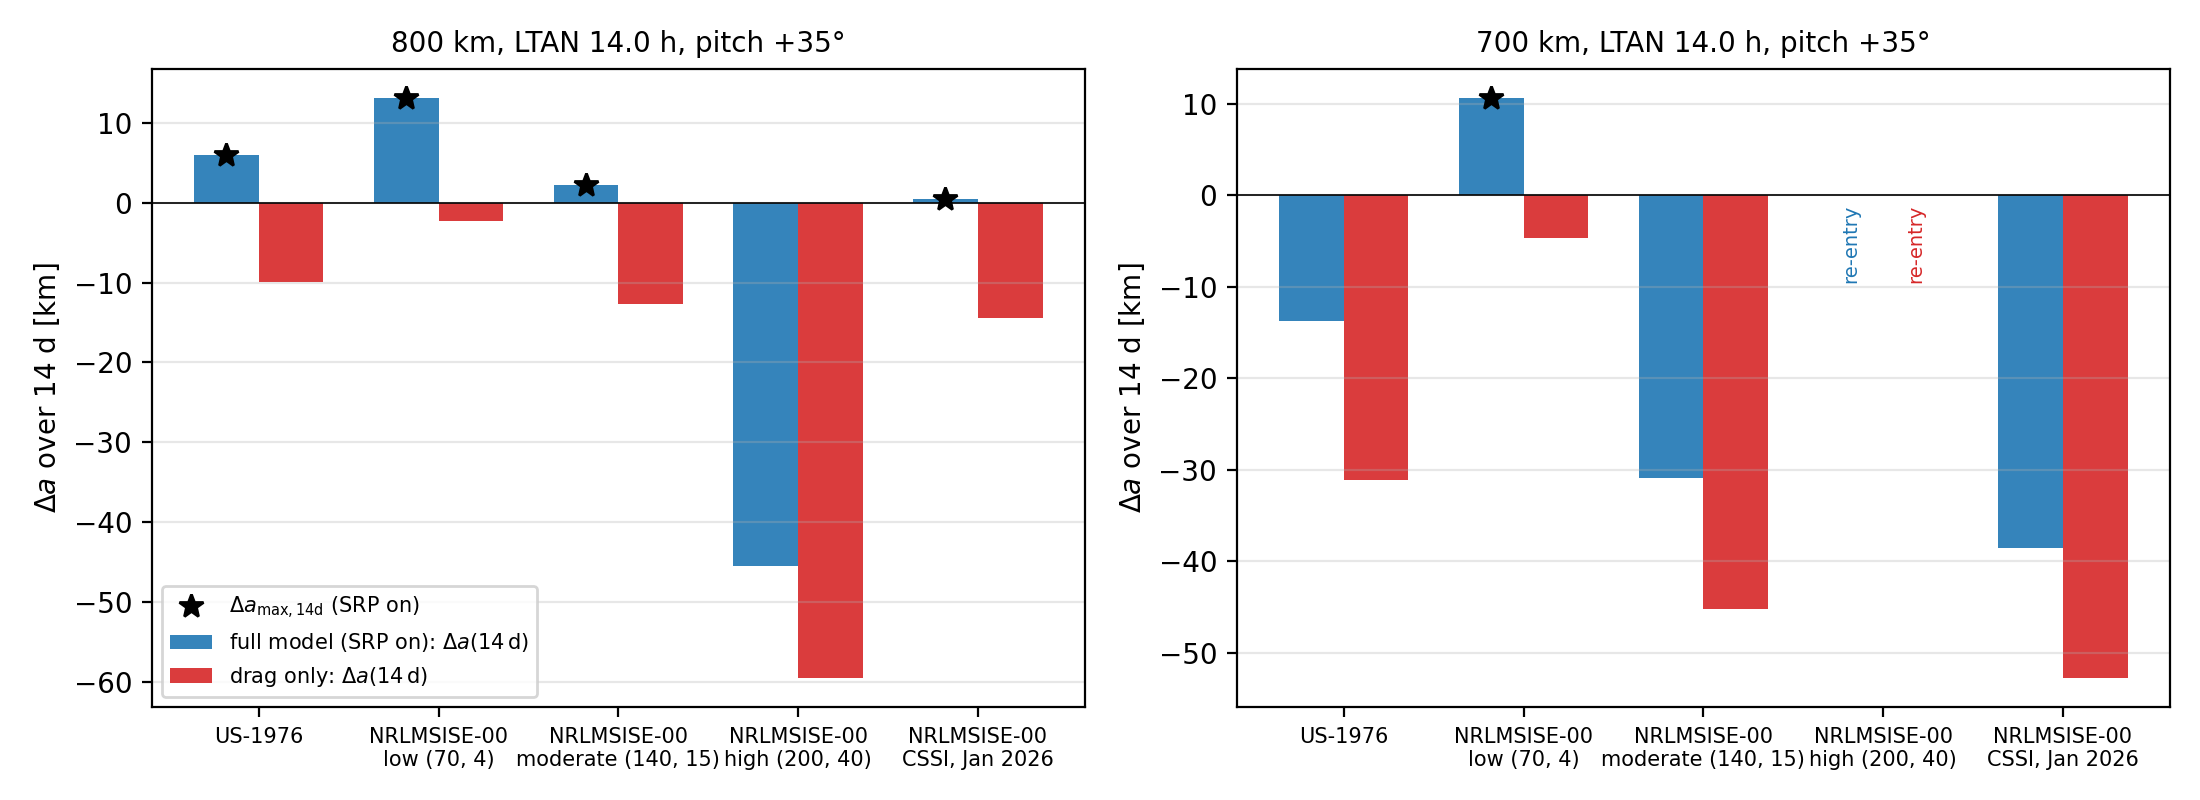
\includegraphics[width=1\linewidth]{Figures/r_space_weather.png}
    \setlength{\abovecaptionskip}{0pt}
    \caption{Space-weather dependence of the \(14\)-day response at the gain-anchor geometry (LTAN \(14.0\,\mathrm{h}\), pitch \(+35^\circ\)) at \(800\,\mathrm{km}\) (left) and \(700\,\mathrm{km}\) (right), from Orekit with DP853 and eclipse event detection. For each atmosphere model --- the US-1976 baseline and NRLMSISE-00 at constant low (\(F_{10.7} = 70\), \(A_p = 4\)), moderate (\(140\), \(15\)) and high (\(200\), \(40\)) activity and with the CSSI space-weather file for January 2026 --- the bars give \(\Delta a(14\,\mathrm{d})\) of the node-sampled mean semi-major axis for the full model (blue) and for drag only (red), and the stars mark \(\Delta a_{\max,14\mathrm{d}}\) of the full model where it is positive. The \(700\,\mathrm{km}\) runs under high activity re-enter within the \(14\) days and are marked ``re-entry''. The gain survives low and moderate activity at \(800\,\mathrm{km}\), is marginal under the January 2026 conditions and closes under high activity; at \(700\,\mathrm{km}\) it exists only under low activity.}
    \label{fig:space_weather}
\end{figure*}

\vspace{5pt}
\par\noindent These results are consistent with the density-multiplier sweep of Section~\ref{sec:sensitivity}, which places the drag-limited boundary at the gain anchor between \(1\times\) and \(2\times\) the US-1976 density at \(800\,\mathrm{km}\) and at or below \(0.5\times\) at \(700\,\mathrm{km}\). Judged by its drag-only decay, the low-activity atmosphere is equivalent to about a quarter of the US-1976 profile at \(800\,\mathrm{km}\) and gives \(+13.18\,\mathrm{km}\), close to the \(13.24\,\mathrm{km}\) of the \(0.25\times\) sweep point; the moderate level and the January 2026 file, at about \(1.3\times\) and \(1.5\times\), fall inside the band and still gain, by \(2.22\) and \(0.50\,\mathrm{km}\), so that the boundary at this geometry lies close to \(1.5\times\) the US-1976 density; high activity, at about \(6\times\), lies far beyond it, as does the Harris--Priester factor of \(3.15\) in Table~\ref{tab:drag_conventions}. At \(700\,\mathrm{km}\) the low-activity atmosphere is equivalent to about \(0.15\times\) the US-1976 profile, below the \(0.5\times\) threshold of the sweep, which is why a gain of \(+10.69\,\mathrm{km}\) appears there and nowhere else at that altitude. The mechanism of Sections~\ref{sec:physics} and \ref{sec:existence} is independent of the atmosphere model; the altitude and activity level at which it becomes net-positive are not, and the quantitative boundary must always be reported together with the atmosphere model and the activity level assumed.

\subsection{Note on the original submission}
\label{sec:val_note}
\noindent The quantitative results of Sections~\ref{sec:existence}--\ref{sec:sensitivity} in the originally submitted version of this paper were produced by a separate implementation of the same model, which was found during revision to contain errors in its aerodynamic incidence-angle convention, in its SRP coefficient and in its solar ephemeris. Those results have been withdrawn. Every result in the present version comes from the open-source propagator of Section~\ref{sec:val_propagator}, after the corrections described in this section, including the correction of the scale heights of the atmosphere table, which is now interpolated exponentially between the tabulated US-1976 values (Section~\ref{sec:model}). The two STK configuration errors of Section~\ref{sec:val_stkconfig} were found by the same read-back procedure, and the gain regime is now realised at \(800\,\mathrm{km}\) rather than at \(700\,\mathrm{km}\), where the corrected model is drag-dominated for every geometry.

\subsection{Data and software availability}
\label{sec:data}
\noindent The open-source propagator, the STK Astrogator build, probe and read-back scripts, the Orekit cross-validation study with its force gates and atmosphere experiments, the plate-definition files, the result files (JSON and NPZ) behind every number in this paper and the scripts that generate every figure and table are archived in the project repository \citep{svarogPropagatorCode2026}, so that the results of this section can be independently reproduced and extended.
\FloatBarrier
